\documentclass[12pt, letterpaper]{report}

%%%%%%%%%%%%%%%%%%
% -- Packages -- %
%%%%%%%%%%%%%%%%%%

% UTF8 encoding
\usepackage[utf8]{inputenc}
\usepackage{bbold}
\usepackage[backend=biber]{biblatex}
\addbibresource{references.bib}

% Graphics and path to graphics
\usepackage{graphicx}
\graphicspath{ {figures/} }
\usepackage{subcaption}

% Colors, especially for highlighting and editing
\usepackage[usenames, dvipsnames]{color}

% Margins, links etc..
\usepackage{float}
\floatplacement{figure}{H}   % Place Figures at same position defined
\usepackage[letterpaper, margin=1in]{geometry}
\usepackage{hyperref}
\hypersetup{
  colorlinks   = true,  %Colours links instead of ugly boxes
  urlcolor     = blue,  %Colour for external hyperlinks
  linkcolor    = black, %Colour of internal links
  citecolor    = black   %Colour of citations
}
\usepackage{setspace}

% Math packages
\usepackage{amsmath}
\usepackage{array}
\usepackage{mathtools}
\usepackage{enumitem}

% Page alignment \addtolength{\hoffset}{0pt}
%\addtolength{\voffset}{0pt}

%%%%%%%%%%%%%%%%%%%%%%%%%%%%%%
% -- Aliases and commands -- %
%%%%%%%%%%%%%%%%%%%%%%%%%%%%%%

\renewcommand{\d}{\delta}       % Dirac delta
\newcommand{\F}{\mathcal{F}}    % Free energy Functional
\renewcommand{\l}{\left}        % Quick left
\renewcommand{\r}{\right}       % Quick right
\newcommand{\f}{\frac}          % Quick fraction
\newcommand{\Z}{\mathcal{Z}}    % GC partition function
\newcommand{\D}{\mathcal{D}}    % Swirly D for path integrals
\newcommand{\fphi}{\tilde{\phi}}% Fourier space phi
\newcommand{\fh}{\tilde{h}}     % Fourier space h
\newcommand{\fxi}{\tilde{\xi}}  % Fourier space xi
\newcommand{\A}{\rho_A}         % Density of species A
\newcommand{\B}{\rho_B}         % Density of species B
\newcommand{\ham}{\mathcal{H}}  % Hamiltonian (classical)
\newcommand{\q}{\mathbf{q}}     % Phase space coordinates
\newcommand{\p}{\mathbf{p}}     % Phase space momenta

% Plane wave + and -
\newcommand{\pwp}{e^{\frac{i\mathbf{p}\cdot\mathbf{q}}{\hbar}}}
\newcommand{\pwm}{e^{-\frac{i\mathbf{p}\cdot\mathbf{q}}{\hbar}}}

% Classical Trace
\newcommand{\trace}[1]{\mathrm{Tr}\left[ #1 \right]}

% Average
\newcommand{\mean}[1]{\left\langle #1 \right\rangle}

% Integral
\newcommand{\integrate}[1]{\int \mathrm{d}#1\,}

% Lazy tilde
\newcommand{\til}{\tilde}

% Tensor and vector symbols
\newcommand*{\tn}[1]{\overline{\overline{#1}}}
\renewcommand*{\vec}[1]{\overline{#1}}

\newenvironment{conditions}
  {\par\vspace{\abovedisplayskip}\noindent\begin{tabular}{>{$}l<{$} @{${}={}$} l}}
  {\end{tabular}\par\vspace{\belowdisplayskip}}

%%%%%%%%%%%%%%%%%%
% Document Begin %
%%%%%%%%%%%%%%%%%%

\pagenumbering{roman}

\begin{document}

%%%%%%%%%%%%%%%%%
%  Front Matter %
%%%%%%%%%%%%%%%%%

\begin{titlepage}
    \begin{center}
        \vspace*{1cm}
        
        \Huge
        \textbf{
            Thesis Title
        }
        
        \vspace{0.5cm}
        \LARGE
        Thesis Subtitle
        
        \vspace{1.5cm}
        \Large 
        \textbf{Nathan Frederick Smith}
        
        \vfill

        \Large
        A thesis presented in partial fulfillment of the degree of\\
        Master's of Science
        
        \vspace{0.8cm}
        
        
\includegraphics[width=0.2\textwidth]{crest.eps}
        
        \Large
        Department of Physics\\
        McGill University, Montreal\\
        Canada\\
        \today
        
    \end{center}
\end{titlepage}



\doublespacing

\section*{Dedication}
\label{sec:dedication}
\addcontentsline{toc}{chapter}{\nameref{sec:dedication}}

This thesis is dedicated to my family and friends. You made this
research and this time in my life possible.


\clearpage

\section*{Acknowledgements}
\label{sec:acknowledgements}
\addcontentsline{toc}{chapter}{\nameref{sec:acknowledgements}}

{
    \color{ForestGreen}
    \begin{itemize}
        \item Nik for a million things
        \item Quentin Stoyel for helping edit
        \item Matt Frick for editing help
        \item Motoki for editing
        \item Paul for editing
    \end{itemize}
}



\clearpage

\section*{Abstract}
\label{sec:abstract}
\addcontentsline{toc}{chapter}{\nameref{sec:abstract}}

Two improvements to the binary Structural Phase Field Crystal (XPFC) theory are
presented. The first is a general phenomenology for modelling density-density
correlation functions and the second extends the free energy of mixing term in
the binary XPFC model beyond ideal mixing to a regular solution model. These
improvements are applied to study kinetics of precipitation from solution. We
see a two-step nucleation pathway similar to recent experimental work
\cite{LOH17, WALLACE13} in which the solution first decomposes into solute-poor
and solute-rich regions followed by nucleation in the solute-rich regions.
Additionally, we find a phenomenon not previously described in literature in
which the growth of precipitates is accelerated in the presence of
uncrystallized solute-rich regions.

\clearpage

\section*{Abrégé}
\label{sec:abrege}
\addcontentsline{toc}{chapter}{\nameref{sec:abrege}}

Nous présentons deux ameliorations au theorie "Structural Phase Field Crystal"
(XPFC) binaire. Le premier decrit une phénoménologie pour une modèle des
fonctions de corrélations des densités, et le deuxième augmente la modèle XPFC
binaire au delà de la modèle idéale en ajutant une terme au énergie libre de
Helmholtz. Ces améliorations sont appliqués aux études kinétiques de la
précipité d'une solution. Nous voyons un chemin de nucléation similaire aux
éxpériments réçentes \cite{LOH17, WALLACE13} dans lequel le solution se sépare
en regions avec concentration de soluté bas et élèvé suivi par nucléation dans
les régions avec hautes concentrations de soluté. De plus, nous decouvrons une
acceleration de l'acroissement du precipité en presence des regions avec une
concentration de soluté élèvé. Ce dernier est une phénomène auparavant pas
décrit en literature. 


\clearpage

\tableofcontents
\listoffigures
\listoftables

\clearpage

\label{sec:list_of_syms}
\addcontentsline{toc}{chapter}{\nameref{sec:list_of_syms}}

\chapter*{List of Symbols}

\begin{description}[labelsep=1cm]
    \item[$\ast$] Denotes an inner product (where appropriate) and
        integration over repeated variables.
    \item[$\mathbf{b}$] Bold font denotes a vector quantity.
    \item[$\beta$] The inverse temperature $1 / k_b T$ where $k_b$ is 
        Boltzmann's constant.
    \item[$\rho$] The average \textit{number} density $N/V$. When refered to as a
        function $\rho(x)$ it is the local number density.
\end{description}


%%%%%%%%%%%%%%%%%%%%%
% -- Main Matter -- %
%%%%%%%%%%%%%%%%%%%%%

\chapter{Introduction}
\pagenumbering{arabic}
\label{chapter:introduction}

% Thesis introduction outline: https://student.unsw.edu.au/introductions

% 1) State the general topic and give some background


% 2) Outline the current situation


% 3) Evaluate the current situation and identify a gap


% 4) Identify the importance of the research (the size of the gap)


% 5) State the research goals and aims


% 6) Outline the order of information


\chapter{Introduction to Classical Density Functional Theory}
\section{Derivation of the General Binary XPFC Free Energy}

In this section we will derive a free energy for a generic binary system starting from basic statistical mechanics.
This will stand as a foundation for many applications we will see later.
To start we consider a single species system and look at the microscopic origins of the PFC free energy functional.
We will see afterwards that generalizing to a multicomponent system relatively simple task.

\subsection{Classical density functional theory for a single component}

In a many body system in which particles interactions are independent of their velocities, we may split contributions to the free energy into two parts: the ideal and the excess.

\subsubsection{The ideal component of the free energy}
The ideal component comes from the kinetic energy term in the Hamiltonian and is known exactly.

\begin{equation}
    \beta\F_{id}[\rho] = \int dr \rho(r) \l\lbrace\ln\right(\Lambda^3\rho(r)\left) - 1\r\rbrace
\end{equation}
Where,
\begin{description}[labelindent=10pt, labelsep=10pt]
\item[$\Lambda^3$] is the thermal DeBroglie volume
\item[$\rho(r)$] is the number density
\item[$\beta$] is the inverse temperature ($1/k_bT$)
\end{description}

\subsubsection{Expansion of the excess free energy}
The excess component comes from the interaction term in the Hamiltonian and is often not known exactly and must be modelled.
A common technique for modelling the excess free energy is to expand it around uniform fluid reference state.
This reference state is characterized by a number density, $\rho_0$, and chemical potential $\mu_0$.

\begin{equation}
    \beta\F_{ex}[\rho] = \beta\F_{ex}^0 +
    \beta\int dr \left.\frac{\d\F_{ex}}{\d\rho}\right\vert_{\rho = \rho_0} \Delta\rho
    + \beta\f{1}{2}\int dr \int dr^\prime \Delta\rho(r^\prime)\l.\f{\d^2\F_{ex}}{\d\rho(r)\d\rho(r^\prime)}\r\vert_{\rho=\rho_0}\Delta\rho(r^\prime) + ...
\end{equation}

Where,
\begin{description}[labelindent=10pt, labelsep=10pt]
    \item[$\Delta\rho$] is difference from reference density ($\rho(r) - \rho_0$)
    \item[$\F_{ex}^0$] is the free energy of the reference state
\end{description}

The excess free energy is the generating function of direct correlation functions $C^(n)(r_1, ..., r_n)$.
In particular this means that direct correlation functions can be written as,

\begin{equation}
    C^{(n)}(r_1, ..., r_n) = -\beta \f{\d^{(n)}\F_{ex}[\rho]}{\d\rho(r_1)...\d\rho(r_n)},
\end{equation}
and our previous expansion can be rewritten in terms of these direct correlation functions.

\begin{equation}
    \beta\F_{ex}[\rho] = \beta\F_{ex}^0 - \int dr C^{(1)}_0(r) \Delta\rho
    + \beta\f{1}{2}\int dr \int dr^\prime \Delta\rho(r^\prime)C^{(2)}_0(r, r^\prime)\Delta\rho(r^\prime) + ...
\end{equation}

In the absence of an external field the single particle direct correlation function of the reference system is simply $\beta\mu^{ex}_0$.

\subsubsection{Total Free Energy}
If we now add in the ideal contribution to the free energy and take advantage of the fact that the excess chemical potential of the reference fluid can be written as the total chemical potential minus the ideal contribution,

\begin{equation}
    \mu^{ex}_0 = \mu_0 - \mu^{id}_0 = \mu_0 - k_bT\ln(\Lambda^3\rho_0).
\end{equation}
to find an expression for the total free energy:

\begin{equation}
    \beta\F[\rho] = \beta\F_0 + \int\,dr \l\lbrace \Delta\rho \ln\l(\f{\Delta\rho}{\rho_0}\r) - (1 - \mu_0)\Delta\rho \r\rbrace
    - \f{1}{2}\int\,dr\int\,dr^\prime \Delta\rho(r) C^{(2)}_0(r, r^\prime) \Delta\rho(r^\prime)
\end{equation}

\subsubsection{Smooth atom approximation and the PFC Free Energy}

To construct the phase-field crystal free energy we assume that the density fluctations, $\Delta\rho(r)$, are small and expand the logarithm term to quartic order in the fluctuations.
Furthermore, we nondimensionalize the free energy by scaling out the reference density, $\rho_0$, and changing variables to $n(r) = \Delta\rho(r)/\rho_0$.

\begin{equation}
    \f{\beta\F[n]}{\rho_0} = \f{\beta\F_0}{\rho_0} +
    \int dr \mu_0 \rho_0 n(r) + \f{n^2(r)}{2} - \f{n^3(r)}{6} + \f{n^4(r)}{12}
    -\f{\rho_0}{2} \int dr \int dr^\prime n(r) C^{(2)}_0(r, r^\prime) n(r^\prime)
\end{equation}

At this point we note that the constant and linear terms in the free energy can be removed without changing the properties of the functional and we are left with the following minimal free energy functional:

\begin{equation}
    \f{\beta\F}{\rho_0} = \int dr \f{n^2(r)}{2} - \f{n^3(r)}{6} + \f{n^4(r)}{12}
    -\f{1}{2} \int dr \int dr^\prime n(r) C^{(2)}(r, r^\prime) n(r^\prime).
\end{equation}

Note, that by convention a factor of the reference density is absorbed into the pair correlation function in the PFC free energy functional.

\subsection{Generalizing the Free Energy to Two Components}
Now that we've seen the recipe for building a phase-field crystal theory for a single component system the process for building a multicomponent theory proceeds analogously with a few minor changes in perspective.
We start again by looking at the ideal and excess contributions to the free energy.

\subsubsection{Ideal Free Energy to Two Components}
The kinetic energy terms of each species in the Hamiltonian give rise to seperate contributions to the free energy as you might expect.
We'll label the two species A and B.

\begin{equation}
    \beta\F^{tot}_{id}[\rho_A, \rho_B] = \beta\F_{id}[\rho_A] + \beta\F_{id}[\rho_B]
\end{equation}
Where,
\begin{description}[labelindent=10pt, labelsep=10pt]
    \item[$\beta\F_{id}$] is the same ideal free energy functional as previously
\end{description}

\subsubsection{Excess Free Energy of a Two Component System}
Our expansion of the excess free energy works just as before but we must sum over the contributions from each species.

\begin{equation}
    \beta\F_{ex} = \beta\F_{ex}^0 - \int \,dr C^{(1)}_{i}(r) \Delta\rho_i(r)
    - \f{1}{2} \int dr \int dr^\prime \Delta\rho_i(r) C^{(2)}_{ij}(r, r^\prime) \Delta\rho_j(r^\prime)
\end{equation}

Where indices denote species (A or B) and repeated indices are summed over.

\subsubsection{Total free energy of a Two Component System}

Putting together the excess and ideal terms together and dropping the constant and linear terms as we did previously we find the following total free energy,

\begin{equation}
    \beta\F[\rho_A, \rho_B] = \int dr \l\lbrace \Delta\rho_i \ln\l(\f{\Delta\rho_i}{\rho_{i0}}\r) - \Delta\rho_i\r\rbrace
        - \f{1}{2} \int dr \int dr^\prime \Delta\rho_i(r) C^{(2)}_{ij}(r, r^\prime) \Delta \rho_j(r^\prime)
\end{equation}

\subsubsection{Changing variables}
Typically, the concentration is the variable we care about in binary systems so instead of preceeding with the usual phase field crystal approximations at this point we make a change of variables to concentration, $c$, and total density, $\rho$.

\begin{align}
    \rho &= \rho_A + \rho_B             & \rho_0 &= \rho_{0A} + \rho_{0B} \nonumber \\
    c &= \f{\rho_A}{\rho_A + \rho_B}    &  c_0 &= \f{\rho_{0A}}{\rho_{0A} + \rho_{0B}} \nonumber
\end{align}

Making this change of variables and seperating total density and concentration contribution we find a free energy functional of the form,

\begin{equation}
    \beta\F[c, \rho] = 
\end{equation}


\chapter{Classical Density Functional Theory of Freezing}
\label{dft_of_freezing}

The classical density functional theories derived in chapter
\ref{fundamentals} was first established to study inhomogenous fluids.
Interestingly, one can think of the solid state as an especially extreme
case of an inhomogeneous fluid \cite{HANSEN-CH6}.  In this case, we can
use CDFT to study the circumstances under which the density field develops
long range periodic solutions (ie., solidification).  While not expressed
in precisely this language, this idea dates back as far as 1941 with the
early work of Kirkwood and Monroe \cite{KIRKWOOD_MONROE41} and was later
significantly refined by Youssof and Ramakrishnan \cite{RAMAKRISHNAN79}.


%%%%%%%%%%%%%%%%%%%%%%%%%%%%%%%%
\section{Amplitude Expansions} %
%%%%%%%%%%%%%%%%%%%%%%%%%%%%%%%%

To explore the problem of solidification, we begin with the approximate grand
potential established in equation \ref{cdft_grand_potential} with the external
potential, $\phi(r)$, set to zero,
%
\begin{equation}
    \beta \Delta \Omega[\rho(r)] =
        \int dr \l\lbrace 
            \rho(r)\ln\l(\f{\rho(r)}{\rho_0}\r) - \Delta\rho(r)\r\rbrace
        - \f{1}{2} \Delta\rho(r) \ast C^{(2)}_0(r, r^\prime)
            \ast \Delta\rho(r^\prime).
\end{equation}
%
Scaling out a factor of $\rho_0$ we can rewrite the grand potential in terms of
a dimensionless reduced density, $n(r) \equiv (\rho(x) - \rho_0)/\rho_0$,
%
\begin{equation}
    \label{gp}
    \f{\beta \Delta \Omega[n(r)]}{\rho_0} =
        \int dr \l\lbrace 
            (1 + n(r))\ln\l(1 + n(r)\r) - n(r)\r\rbrace
        - \f{1}{2} n(r) \ast \rho_0 C^{(2)}_0(r, r^\prime) \ast n(r^\prime).
\end{equation}
%
To describe the density profile in the solid state we can expand the density
in a plane waves,
%
\begin{equation}
    \label{expansion}
    n(r) = \bar{n} + \sum_{\mathbf{G}} \xi_{\mathbf{G}} e^{i \mathbf{G} r}.
\end{equation}
%
Where, $\l\lbrace \mathbf{G} \r\rbrace$, is the set of reciprocal lattice
vectors in the crystal lattice and the amplitudes, $\xi_\mathbf{G}$, serve as
order parameters for freezing. In the liquid phase all amplitudes are zero and
the average density is uniform, while in the solid phase there are finite
amplitudes that describe the periodic profile of the crystal lattice. Setting
the liquid at the melting point as our reference fluid we find that, at the 
melting point, $\bar{n}$ is zero for the liquid and is the fractional density
change of solidification, $(\rho_s - \rho_l)/\rho_l$, in the solid phase.

The amplitudes are constrained by the point group symmetry of the lattice.
Grouping the amplitudes of symmetry-equivalent reciprocal lattice vectors
together we can write the density profile as,
%
\begin{equation}
    \label{amplitudes}
    n(r) = \bar{n}
         + \sum_\alpha \l\lbrace
            \xi_\alpha \sum_{\lbrace\mathbf{G}\rbrace_\alpha}
                e^{i\mathbf{G} \cdot \mathbf{x}}\r\rbrace,
\end{equation}
%
Where $\alpha$ is a label running over sets of symmetry-equivalent reciprocal
lattice vectors.

If we insert equation \ref{amplitudes} into equation \ref{gp} and integrate
over the unit cell we find,
%
\begin{align}
    \label{amplitude_gp} 
    \f{\beta \Delta\Omega_{cell}}{\rho_0} &=  \int_{cell} 
        dr \l\lbrace (n(r) + 1)\ln\l(n(r) + 1\r) - n(r) \r\rbrace \nonumber \\
    &- \f{1}{2} \l[\bar{n} ^ 2 \rho_0\tilde{C}^{(2)}_0(0) + \sum_\alpha\rho_0\tilde{C}^{(2)}_0
            (\mathbf{G}_\alpha) \lambda_\alpha\vert\xi_\alpha\vert^2\r],
\end{align}
%
Where $\lambda_\alpha$ is the number of reciprocal lattice vectors in the set
$\alpha$ and $\tilde{C}^{(2)}_0(k)$ is the Fourier transform of the direct
correlation function of the reference fluid. The first term in equation
\ref{amplitude_gp} is convex in all of the amplitudes with a minimum at zero.
It follows that solidification must occur when the direct correlation function
at the reciprocal lattice vectors, $\tilde{C}^{(2)}_0(\mathbf{G}_\alpha)$, is
large enough to stabilize a finite amplitude by creating a new minimum away
from zero.

Furthermore, equation \ref{amplitude_gp} suggests that this transition depends
only on a set of parameters, $\rho_0 \tilde{C}^{(2)}_0(\mathbf{G}_\alpha)$,
that are material independent.  That is to say, once we specify the symmetry of
the lattice a liquid will solidify into (eg.  face-centred-cubic), all
materials that undergo this transition should share these parameters at the
melting point. This seems to be the case for a variety of materials. For
instance, for many liquids solidifying into face-centred-cubic (fcc) lattices,
these parameters for the [111] and [311] reciprocal lattice vectors are 0.65
and 0.23 respectively. Similarly, for a spectrum of liquids solidifying into
body-centred-cubic (bcc) lattices these parameters  for the [110] and [211]
reciprocal lattice vectors are approximately 0.66 and 0.12 respectively.

As seen in table \ref{table:ramakrishnan_argon} and table
\ref{table:ramakrishnan_sodium} theoretical results from this approach match
very closely to experimental values. In spite of the successes of density
functional approach pioneered by Youssof and Ramakrishnan there are limits
to this framework.

\begin{table}[]
    \center
    \begin{tabular}{l c c c}
        \hline 
        Theory & $\tilde{C}(\mathbf{G}_{[111]})$ & $\tilde{C}(\mathbf{G}_{[311]})$ & $\bar{n}$ \\ 
        \hline
        I & 0.95 & 0.0 & 0.074 \\
        II & 0.65 & 0.23 & 0.270 \\
        III & 0.65 & 0.23 & 0.166 \\
        Experiment & 0.65 & 0.23 & 0.148\\
        \hline
    \end{tabular}
    \caption[Freezing parameters for Argon]{Freezing parameters for Argon (fcc)
    taken from \cite{RAMAKRISHNAN79}.  Theory I uses one order paramter, theory
    II uses two order parameters and theory III uses two order parameters and
    expands to third order in the free energy. $\eta$ is the fractional density
    change of solidification 
    $(\rho_s - \rho_l) / \rho_l)$.}
    \label{table:ramakrishnan_argon}
\end{table}

\begin{table}[]
    \center
    \begin{tabular}{l c c c}
        \hline 
        Theory & $\tilde{C}(\mathbf{G}_{[110]})$ & $\tilde{C}(\mathbf{G}_{[211]})$ & $\bar{n}$ \\ 
        \hline
        I           & 0.69 & 0.00 & 0.048 \\
        II          & 0.63 & 0.07 & 0.052 \\
        III         & 0.67 & 0.13 & 0.029 \\
        Experiment  & 0.65 & 0.23 & 0.148\\
        \hline
    \end{tabular}
    \caption[Freezing parameters for Sodium]{Freezing parameters for Sodium
    (bcc) taken from \cite{RAMAKRISHNAN79}.  Theory I uses one order paramter,
    theory II uses two order parameters and theory III uses two order
    parameters and expands to third order in the free energy. $\eta$ is the
    fractional density change of solidification 
    $(\rho_s - \rho_l) / \rho_l)$.}
    \label{table:ramakrishnan_sodium}
\end{table}

Many of the mechanical properties of solids are due to the way in which they
deviate from the perfect crystalline lattice: the microstructure. Grain
boundaries, vacancies, dislocations and second phase particles all play
critical roles in determining the mechanical properties of solids. A simple
example of this is the Hall-Petch effect which states that the yield stress of
a material increases with decreasing grain size,
%
\begin{equation}
    \sigma = \sigma_0 + k_y d^{-1/2},
\end{equation}
%
where, $d$, is the average grain diameter, $\sigma$ is the yield stress,
$\sigma_0$ is yield stress of a single crystal sample and $k_y$ is the
strengthening coefficient.

Microstructure plays key roles not only in the mechanical properties but also
the kinetic pathways of certain phase transformations. For instance,
dislocations can act to catalyze precipication in binary alloys [cite Vahid].

The problem that we face is then, how do we examine these defects and
microstructural elements but retain some of the successful aspects of density
functional approach? One way to think about to consider the microstructure in
the solid state is that it is an artifact of not having fulling reached
equilibrium. Real materials are solidified over a finite time and therefore
haven't fully reached equilibrium. As a result, we should study the pathway to 
equilibrium to gain insight into the origin of microstructure. 

%%%%%%%%%%%%%%%%%%%%%%%%%%%%%%%%%%%%%%%%%%%%%
\section{Dynamic Density Functional Theory} %
%%%%%%%%%%%%%%%%%%%%%%%%%%%%%%%%%%%%%%%%%%%%%

Using techniques from non-equilibrium statistical mechanics we can extend
the density functional approach to a dynamic model. To start we illustrate the 
non-equilibrium method schematically. Consider a non-equilibrium probability 
distribution over phase space, $f(\q, \p; t)$. As a function over phase space,
its equation of motion is a simple result of classical mechanics,
%
\begin{equation}
    \label{cm} 
    \f{d f}{dt} = \l\lbrace f, \mathcal{H} \r\rbrace + \f{\partial f}{\partial t}.
\end{equation}
%
Where, $\l\lbrace \cdot, \cdot \r\rbrace$, denotes the Poisson bracket,
%
\begin{equation}
    \l\lbrace f, g \r\rbrace = \sum_{i = 0}^N \f{\partial f}{\partial q_i}
        \f{\partial g}{\partial p_i} - \f{\partial g}{\partial q_i}
        \f{\partial f}{\partial p_i}.
\end{equation}
%
Of course, the distribution must remain normalized in time and therefore the 
total time derivative must be zero,
%
\begin{equation}
    \int d\q d\p\, f(\q, \p; t) = 1 \rightarrow \f{d f}{dt} = 0.
\end{equation}
%
Accounting for this conservation law in equation \ref{cm}, the resulting
equation of motion is called the \textit{Liouville Equation},
%
\begin{equation}
    \label{liouville} 
    \f{\partial f}{\partial t} = - \l\lbrace f , \mathcal{H} \r\rbrace
\end{equation}
%
Under appropriate conditions the probability distribution, under the action of
the Liouville Equation, will decay to a stable fixed point $f_{eq}(\q, \p)$ we
call equilibrium,
%
\begin{equation}
    \lim_{t \rightarrow \infty} f(\q, \p; t) = f_{eq}(\q, \p)
\end{equation}
%

Using the non-equilibrium probability distribution, we can also discuss
non-equilibrium averages of the density profile and their associated equations
of motions. The non-equilibrium density is written in analogy with equation
\ref{mean_density} by taking of the classical trace of the density operator
over with the non-equilibrium distribution,
%
\begin{equation}
    \rho(x, t) = \mean{\hat{\rho}(x; \q)}_{ne} =
        \trace{\hat{\rho}(x; \q) f(\q, \p, t)}.
\end{equation}
%
Where, $\mean{\cdot}_{ne}$, denotes the non-equilibrium average. Just as the
non-equilibrium probability distribution is driven to equilibrium by the
Liouville Equation, so too is the density profile by its own equation of
motion.

A variety of equations of motion for the density field are known.  For
instance, we can consider the Navier-Stokes equations of hydrodynamics to one
such equation of motion. If we restrict ourselves to diffusion limited
circumstances, we may derive a much simplier equation of motion. To acheive
this result we use the projection operator method, and assume that the 
density operator is the only relevant variable. Quoting the result from
\cite{ESPANOL09} we find,
%
\begin{equation}
    \label{eq:mean_eom}
    \f{\partial \rho(x, t)}{\partial t} = 
        \nabla \cdot \integrate{r^\prime} \mathbf{D}(r, r^\prime, t) 
        \cdot \nabla^\prime \f{\d \F[\rho]}{\d \rho(x^\prime, t)},
\end{equation}
%
Where, $\mathbf{D}(r, r^\prime, t)$, is the diffusion tensor,
%
\begin{equation}
    \mathbf{D}(r, r^\prime, t) = \int_0^\infty \mathrm{d}\tau^\prime\,
        \trace{f(\q, \p, t)\hat{\mathbf{J}}(r, 0)
        \hat{\mathbf{J}}(r^\prime, \tau^\prime)},
\end{equation}
%
in which $\mathbf{J}(r, t)$ is the density flux is,
%
\begin{equation}
    \hat{\mathbf{J}}(r, t) \equiv 
        \sum_i^N \frac{p_i}{m_i} \d(q_i - r).
\end{equation}

Should we use assume 

{
    \color{ForestGreen}

If we restrict ourselves to the case where
transport is diffusion limited and we assume that the dynamic pair correlation
function is the same as the equilibrium pair correlation we can express the
density equation of motion as,
%
\begin{equation}
    \label{mean_eom}
    \f{\partial \rho(x, t)}{\partial t} = 
        \nabla \cdot \l[
            D_0 \rho(x, t) \nabla \l(\f{\d \F[\rho]}{\d \rho(x, t)}\r)
        \r].
\end{equation}
%
Where, $D_0$ is the diffusion constant. We can also express the dynamics of
the density field in the form of a Langevin equation for the density operator,
%
\begin{equation}
    \label{langevin_eom}
    \f{\partial \hat{\rho}(x, t)}{\partial t} =
        \nabla \cdot \l[
            D_0 \hat{\rho}(x, t) \nabla \l(\f{\d \F[\hat{\rho}]}{\d \hat{\rho}}\r)
        \r] + \xi(x, t).
\end{equation}
%
Where, $\mathbf{\xi}(x, t)$ is a Gaussian random driving force with zero mean
and variance of,
%
\begin{equation}
    \mean{\xi(x, t)\xi(x^\prime, t^\prime)} = -2 \nabla \cdot \l[ D_0 \rho(x,t) 
        \nabla \d(x - x^\prime) \d(t - t^\prime)
    \r],
\end{equation}
%
Due to a generalized Einstein relation\footnote{See Appendix \ref{noise} for
details on generalized Einstein relations for nonlinear Langevin equations} for
the Langevin equation in equation \ref{langevin_eom}.

Equation \ref{mean_eom} and \ref{langevin_eom} were first derived by Marconi
and Tarazona by considering an ensemble of interacting Brownian particles, but
other derivations are possible including the projection operator method [cite
Espanol].  Equations \ref{mean_eom} and \ref{langevin_eom} fall under the
heading of \textit{Dynamic Density Functional Theory} (DDFT) or sometimes
\textit{Time dependent density functional theory} (TD-DFT) though we'll use the
former throughout this text.
}

Unfortunately, if we were to use the approximate free energy functional
established in equation \ref{cdft_free_energy} in the dynamic density
functional theory of equation \ref{mean_eom} or \ref{langevin_eom} we would
face a major impedement: the solid state solutions of the density functional
theory approach yield sharply peaked solutions at the position of the atoms in
the lattice. While this is realistic, they are a major challenge for numerical
algorithms. The challenges are two fold: first, these sharp peaks require a fine mesh 
to be resolved resulting in large memory requirement to simulate domains 
of any non-trivial scale and second, lineary stability analysis of most algorithms 
slave the scale of the time step to the scale of the grid spacing so only small
time steps can be taken on a fine mesh.

%%%%%%%%%%%%%%%%%%%%%%%%%%%%%%%%%%%%%%
\section{Phase Field Crystal Theory} %
%%%%%%%%%%%%%%%%%%%%%%%%%%%%%%%%%%%%%%

The phase field crystal theory (PFC) presents a solution to the numerical difficulties
faced by DDFT methods by approximating the free energy in such a say as to retain the
basic features of the theory with a smoother solid state solution. Starting the 
approximate free energy functional of equation \ref{cdft_free_energy} we proceed as
previously by scaling out a factor of the reference density and changing variables
to a dimensionless density $n(r) = (\rho(r) - \rho_0) / \rho_0$,
%
\begin{equation}
    \f{\beta \F[n(r)]}{\rho_0} = 
        \int dr \l\lbrace (n(r) + 1) \ln( n(r) + 1) - (1 - \beta\mu)n(r) \r\rbrace
        - \f{1}{2} n(r) \ast \rho_0 C^{(2)}_0(r, r^\prime) \ast n(r^\prime).
\end{equation}
%
We then Taylor expand the logarithm about the reference density or equivalently
$n(r) = 0$, to fourth order,
%
\begin{equation}
    \label{pfc_free_energy} 
    \f{\beta \F[n(r)]}{\rho_0} =
        \int dr \l\lbrace \f{n(r)^2}{2} - \f{n(r)^3}{6} + \f{n(r)^4}{12} \r\rbrace
        -\f{1}{2} n(r) \ast \rho_0 C^{(2)}_0(r, r^\prime) \ast n(r^\prime).
\end{equation}
%
Where the linear term has been dropped because it leaves the equations of
motion invariant.  Most phase field crystal theories also use a simplified
equation of motion as well,
%
\begin{equation}
    \label{pfc_eom}
    \f{\partial n(r, t)}{\partial t} = M \nabla^2 \l(\f{\d \F[n(r)]}{\d n(r)}\r).
\end{equation}
%


\chapter{Simplified Binary Phase Field Crystal Models}
In this chapter we will walk through three simplified binary PFC models. The
first is the original binary PFC model, which, while highly successful at
modelling a few important phenomena is ultimately limited in scope. The second
is the binary structural phase field crystal, or binary XPFC which was
successful in modelling a broad spectrum of crystalline structures, but was
limited in its ability of model liquid instablilities and a variety of phase
diagrams. Finally, we'll see a new contribution to which we will call the
regular phase field crystal model which is successful in modeling a broad
spectrum of invariant binary reactions and crystalline structures. 

\section{Original Binary Phase Field Crystal Model}

To derive the original binary PFC model, we begin with a multicomponent variant of
equation \ref{cdft_free_energy}, 
%
\begin{align}
    \beta\F[\A, \B] &= \sum_{i=A, B} \int \mathrm{d}r \rho_i \ln\l(\f{\rho_i}{\rho_i^0}\r) 
            - (1 - \mu_i^0) \Delta\rho_i \\
        &- \f{1}{2} \sum_{i,j=A, B} \int \mathrm{d}r \mathrm{d}r^\prime \Delta\rho_i(r) 
            C^{(2)}_{ij}(r, r^\prime) \Delta\rho_j(r^\prime).
\end{align}
%
As noted in chapter \ref{dft_of_freezing}, we can produce a PFC model by approximating
the ideal component of the free energy. 

\section{Binary Structural Phase Field Crystal Model}

\section{Regular Phase Field Crystal Model}

\section*{Derivation of the General Binary XPFC Free Energy}

Now that we've seen the recipe for building a phase-field crystal theory for a
single component system the process for building a multicomponent theory
proceeds analogously with a few minor changes in perspective.  We start again
by looking at the ideal and excess contributions to the free energy.

\subsubsection{Ideal Free Energy to Two Components} The kinetic energy terms of
each species in the Hamiltonian give rise to seperate contributions to the free
energy as you might expect.  We'll label the two species A and B.

\begin{equation} \beta\F^{tot}_{id}[\rho_A, \rho_B] = \beta\F_{id}[\rho_A] +
\beta\F_{id}[\rho_B] \end{equation} Where,
\begin{description}[labelindent=10pt, labelsep=10pt] \item[$\beta\F_{id}$] is
            the same ideal free energy functional as previously
\end{description}

\subsubsection{Excess Free Energy of a Two Component System} Our expansion of
the excess free energy works just as before but we must sum over the
contributions from each species.

\begin{equation} \beta\F_{ex} = \beta\F_{ex}^0 - \int \,dr C^{(1)}_{i}(r)
\Delta\rho_i(r) - \f{1}{2} \int dr \int dr^\prime \Delta\rho_i(r)
C^{(2)}_{ij}(r, r^\prime) \Delta\rho_j(r^\prime) \end{equation}

Where indices denote species (A or B) and repeated indices are summed over.

\subsubsection{Total free energy of a Two Component System}

Putting together the excess and ideal terms together and dropping the constant
and linear terms as we did previously we find the following total free energy,

\begin{equation} \beta\F[\rho_A, \rho_B] = \int dr \l\lbrace \Delta\rho_i
\ln\l(\f{\Delta\rho_i}{\rho_{i0}}\r) - \Delta\rho_i\r\rbrace - \f{1}{2} \int dr
\int dr^\prime \Delta\rho_i(r) C^{(2)}_{ij}(r, r^\prime) \Delta
\rho_j(r^\prime) \end{equation}

\subsubsection{Changing variables} Typically, the concentration is the variable
we care about in binary systems so instead of preceeding with the usual phase
field crystal approximations at this point we make a change of variables to
concentration, $c$, and total density, $\rho$.

\begin{align} \rho &= \rho_A + \rho_B             & \rho_0 &= \rho_{0A} +
\rho_{0B} \nonumber \\ c &= \f{\rho_A}{\rho_A + \rho_B}    &  c_0 &=
\f{\rho_{0A}}{\rho_{0A} + \rho_{0B}} \nonumber \end{align}

Making this change of variables and seperating total density and concentration
contribution we find a free energy functional of the form,

\begin{equation} \beta\F[c, \rho] = \end{equation}


\chapter{Improvements to the Binary XPFC Model}
\label{chapter:improvements}

All my improvements


\chapter{Applications}
\label{chapter:applications}

In this chapter we discuss applications of our improvements to the binary XPFC
model.  To begin we'll discuss an effective equation of motion in the limit
that density change on solidification is small, after which we'll examine the
to process of multi-step nucleation of nanoparticles from solution. To conclude
we'll discuss areas of future application.

%%%%%%%%%%%%%%%%%%%%%%%
\subsection{Dynamics} %
%%%%%%%%%%%%%%%%%%%%%%%

To examine applications of our improvements to the XPFC model we begin by
considering equations of motion. Following \cite{GREENWOOD11_BINARY}, we use
conservative dynamics for both $n(x, t)$ and $c(x, t)$.
%
\begin{gather}
    \f{\partial n(x, t)}{\partial t} = 
        M_n \nabla^2\l(\f{\d \beta \Delta\F / \rho_0}{\d n(x, t)}\r) 
        + \xi_n(x, t), \\ 
    \f{\partial c(x, t)}{\partial t} = 
        M_c \nabla^2\l(\f{\d \beta \Delta \F / \rho_0}{\d c(x, t)}\r)
        + \xi_c(x, t).
\end{gather}
%
These equations of motion are largely phenomenological as, strictly speaking,
there is no reason that the local concentration should be conserved.  This
conservation can be justified in the limit that the total density does not
deviate far from the reference. When this is the case we have $c \equiv \B /
\rho \approx \B / \rho_0$ which \textit{is} conserved.

%%%%%%%%%%%%%%%%%%%%%%%%%%%%%%%%%%%%%%%%%%%%%%%%%%%%%%%%%%%%%
\section{Multistep Nucleation of Nanoparticles in Solution} %
%%%%%%%%%%%%%%%%%%%%%%%%%%%%%%%%%%%%%%%%%%%%%%%%%%%%%%%%%%%%%

Recent experimental work has shown that precipitation of nanoparticles solution
can follow a pathway vary different from that assumed by Classical Nucleation
Theory (CNT).  In gold and silver nanoparticles\cite{LOH17} as well as calcium
carbonate (CaCO${}_3$)\cite{WALLACE13} systems precipitation occurs first via
spinodal decomposition of the aqueous solution followed by nucleation inside
the resulting solute-rich liquid droplets. CNT assumes that, for binary
systems, assumes that changes in order and composition occur simultaneously.
While there is some dispute about whether or not to call this process a
non-classical nucleation pathway \cite{DAVEY13, GEBAUER11}, the observed pathway
to precipitation raises several questions regardless of semantics about its
classification. Under what conditions does this pathway occur? How does the 
pathway effect the polydispersity of the final nanoparticle? We present here
initial finding using the improved binary XPFC formalism.

These experimental findings are among many works that point to a deficiency in
CNT. Common among these works is the presence of a multi-step nucleation
process. While some theoretical description exist for these multi-step
processes, they typically posit highly simplified pathways to nucleation for
simplicity of analysis that may be far from the actual kinetics experienced by
the system.  For instance in the study of condensation of a pure material,
Lutsko \textit{et al.} \cite{LUTSKO15} restricted the nucleus to a spherical
droplet with radius $R$ and density $\rho$. Thus restricted, they find that the
most likely path to nucleation follows a three-stage pathway.  These theories
can justify a multi-step nucleation pathway but do little more to advance our
knowledge of the \textit{actual} pathway to nucleation.

It is important, then, to have robust models that contain all of the essential
physics of these systems to gain a deeper insight into the phenomena. The works
of Loh \cite{LOH17} are a special case of diffusion limited precipitation because
their system was a 30nm thick aqueous solution. The effective diffusion
constant in this thin water film is 9 orders of magnitude smaller than in the
bulk and as such the system is diffusion limited. To model this process we must
be able to  model changes in composition, structure and density. A negative
enthalpy of mixing is clearly playing in important role so our improved XPFC
model is a good fit.

To construct an appropriate free energy functional for this system we consider
the structure of its equilibrium phase diagram. Precipitation is indicative of
a simple liquid-solid coexistance curve beneath which we assume there also a
submerged metastable liquid spinodal \cite{DAVEY13}. Producing a system with
these characteristics is similar to that of a monotectic with the exception
that the spinodal temperature, $T_c$, must now be sufficiently low to hide
below the coexistance curve. We will also also use a Gaussian window function
$\zeta(c)$ as the in the monotectic case though this time centring the Gaussian
about $c = 1$ in keeping with interpreting the concentration as a solute
concentration.  An example, including depiction of the metastable spinodal, can
be seen in figure \ref{fig:precip_phase_dia}.

\begin{figure}
    \centering	
    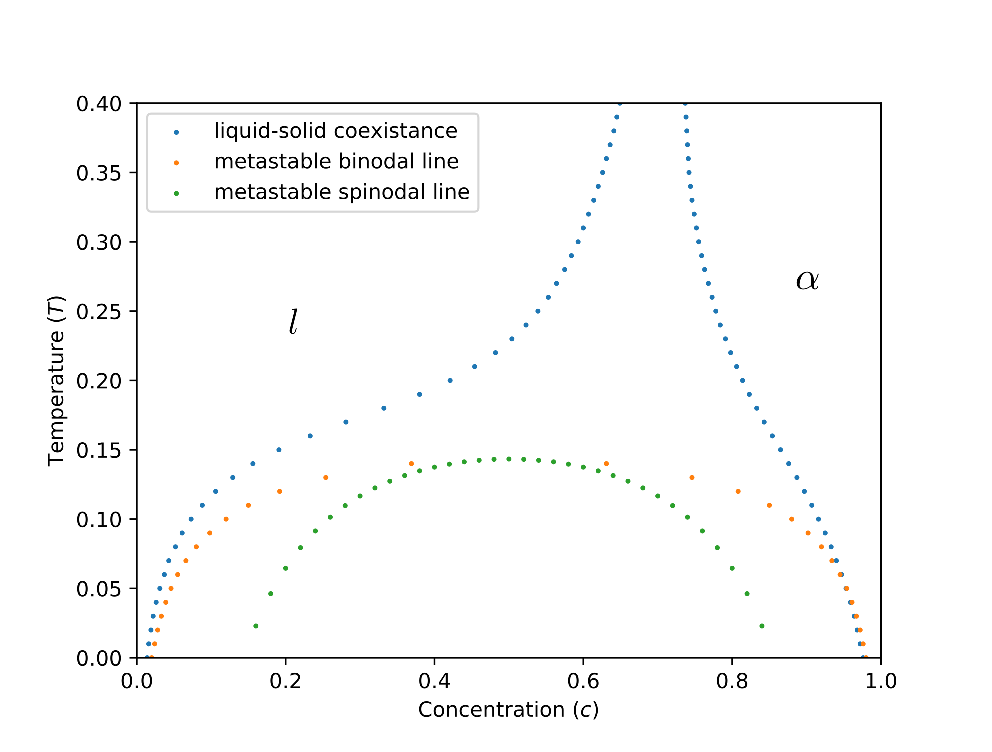
\includegraphics[scale=0.8]{solution.eps}
    \caption[Coexistance Phase Diagram with Metastable Spinodal]{
        \label{fig:precip_phase_dia} Phase Diagram of a Precipitating Solution
        with hexagonal $\alpha$ phase. The free energy parameters are $\eta =
        2$, $\chi = 1$, $\omega=0.3$, $\epsilon_0=30$, $T_c = 0.15$ and
        $c_0=0.5$. The parameters for the base correlation function are
        $\sigma_{10\alpha} = 0.8$, $k_{10\alpha} = 2\pi$, and $T\_0 = 1$ and
        the parameters for the interpolation function are $\sigma_c = 0.5$.
    }
\end{figure}

We would expect that, starting from a uniform initial condition, if we quench
the system through the coexistance region and past the liquid spinodal we might
see a nucleation pathway similar to that observed experimentally. Results of a
numerical simulation \footnote{See appendix \ref{appendix:algorithm} for a
detailed description of the integration algorithm} can be seen in figure
\ref{fig:precipitation}. We see that, much as in experimental observation,
nanoparticle nucleation is preceded by spinodal decomposition.

\begin{figure}
    \centering
    \begin{subfigure}[b]{0.3\textwidth}
        \includegraphics[width=\textwidth]{initial}
        \label{fig:initial}
        \caption{}
    \end{subfigure}
    ~
    \begin{subfigure}[b]{0.3\textwidth}
        \includegraphics[width=\textwidth]{early_spinodal}
        \label{fig:early_spinodal}
        \caption{}
    \end{subfigure}
    ~
    \begin{subfigure}[b]{0.3\textwidth}
        \includegraphics[width=\textwidth]{devel_spinodal.png}
        \label{fig:devel_spinodal}
        \caption{}
    \end{subfigure}

    \vspace{0.25cm}
    \begin{subfigure}[b]{0.3\textwidth}
        \includegraphics[width=\textwidth]{nucleation}
        \label{fig:nucleation}
        \caption{}
    \end{subfigure}
    ~
    \begin{subfigure}[b]{0.3\textwidth}
        \includegraphics[width=\textwidth]{nucleation_and_sacrificial_growth}
        \label{fig:nucleation_and_growth}
        \caption{} 
    \end{subfigure}
    ~
    \begin{subfigure}[b]{0.3\textwidth}
        \includegraphics[width=\textwidth]{sacrificalgrowth}
        \label{fig:sacrifical_growth}
        \caption{}
    \end{subfigure}
    
    \vspace{0.25cm}
    \begin{subfigure}[b]{0.3\textwidth}
        \includegraphics[width=\textwidth]{crystalgrowth}
        \label{fig:crystalgrowth}
        \caption{}
    \end{subfigure}
    ~
    \begin{subfigure}[b]{0.3\textwidth}
        \includegraphics[width=\textwidth]{crystalgrowth2}
        \label{fig:crystalgrowth2}
        \caption{}
    \end{subfigure}
    ~ 
    \begin{subfigure}[b]{0.3\textwidth}
        \includegraphics[width=\textwidth]{crystalgrowth3}
        \label{fig:crystalgrowth3}
        \caption{}
    \end{subfigure}
    \caption[Stages of precipitation of nanoparticles from solution]{
        \label{fig:precipitation}
        Various stages of precipitation of nanoparticles from solution. All
        thermodynamic parameters are shared with figure
        \ref{fig:precip_phase_dia}. The initial condition is a uniform solution
        quenched abruptly to $T$ = 0.07. The initial condition has
        concentration $c = 0.3$ and relative density $n = 0.05$. Mobilities
        $M_n$ and $M_c$ are set to 1 and $W_c$ is set to 3.0. Numerical
        parameters are grid spacing $\Delta x = 0.125$ on a 1024 by 1024
        lattice with time step size $\Delta t = 0.0025$. Sub-figures (a) - (c)
        show spinodal decomposition of the liquid into solute right and solute
        poor regions. Sub-figures (d) - (f) show nucleation of the solid and
        solid growth at the expense of liquid regions.  The remaining
        sub-figures show only nanoparticle growth and coarsening.
    }
\end{figure}

Our model finds some addition complexity in the nucleation process as well.
Once crystalline nuclei start to form, they growth is accelerated at the
expense of the solute-rich liquid droplets in solution. In a system of coarsen
droplets with only a single phase, larger droplets grow at the expense of
smaller droplets to reduce the total surface tension in the system. This
process is called Oswald ripening. In the nanoparticle system even smaller
crystalline particles can grow at the expense of larger liquid droplets due to
their difference in chemical potential.

\begin{figure}
    \centering
    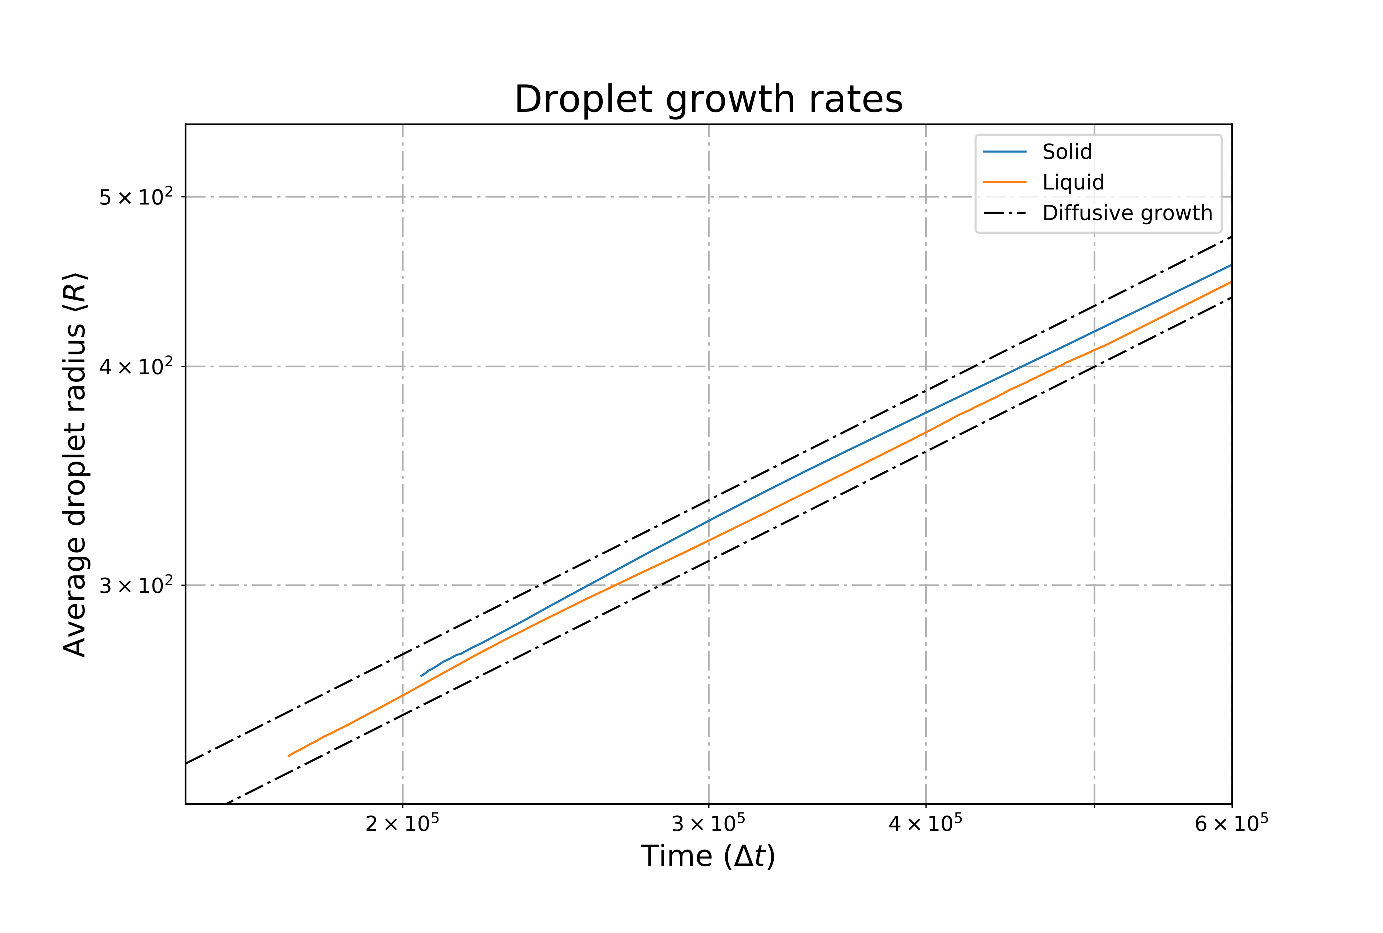
\includegraphics[width=\textwidth]{scaling}
    \caption{
        \label{fig:scaling}
        Droplet growth exponents
    }
\end{figure}

We can examine this growth phenomena more systematically by measuring the
ensemble average droplet radius $\langle R(t) \rangle$ over time. We achieve
this by running 120 simulations with the same parameters as the quench
described in figure \ref{fig:precipitation} and computing the radius of all
droplets and their phase (liquid or solid) throughout the simulation. Strictly
diffusive growth scales like $\mean{R(t)} \sim t^{1/2}$ and so in plotting the
mean radius versus time on a log-log plot as in figure \ref{fig:scaling} we see
how the growth of solid and liquid droplets compare to diffusive growth. Early
solid droplets grow at a weakly hyper-diffusive rate due to the presence of
the sacrificial liquid droplets and slow to sub-diffusive as they begin to
coarsen.

\begin{figure}
    \centering
    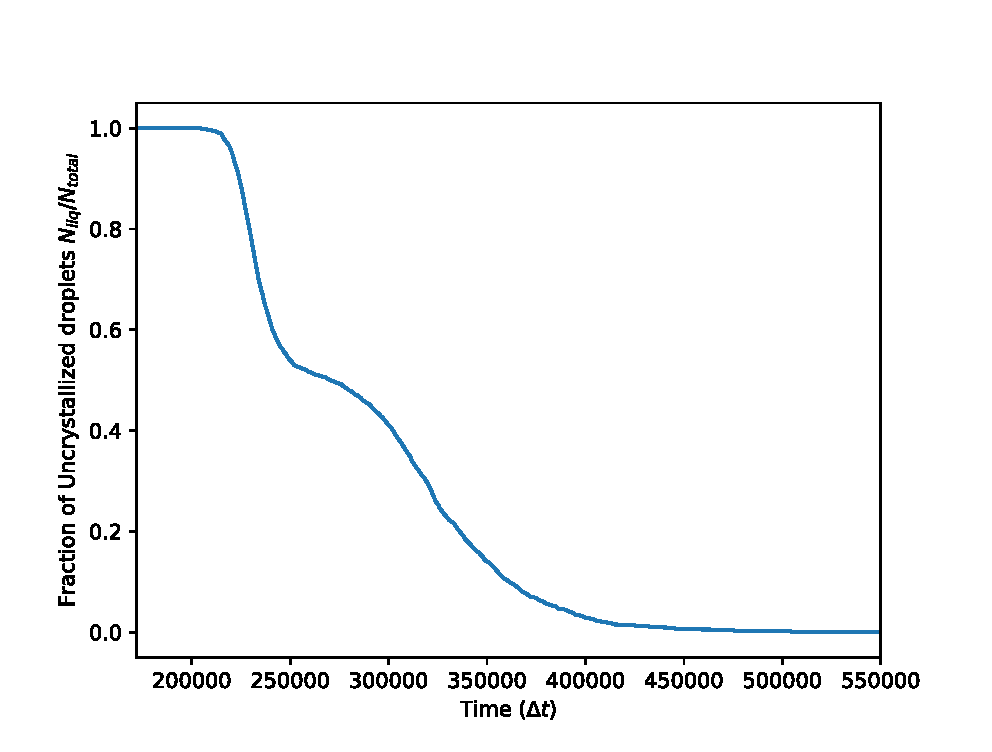
\includegraphics[width=0.7\textwidth]{incubation}
    \caption[Fraction of uncrystallized droplets in time]{
        \label{fig:incubation}
        Fraction of uncrystallized droplets in time
    }
\end{figure}

A more pronounced view of this phenomena can be seen by examining the fraction
of uncrystallized droplets in the system with respect to time as in figure
\ref{fig:incubation}. Neither classical nor proposed non-classical nucleation
theories explain the pronounced reduction in nucleation rate seen once the
fraction of solid droplets reachs approximately one half. Instead of developing
via nucleation in the remaining droplets we see liquid droplet anhilation
beginning to become an important driving factor in increasing the solid
fraction. As liquid droplets shrink the nucleation rate inside the droplet is
suppressed by solute and density segregation to solid droplets. In classical
nucleation theory we would expect an exponential decay and even in proposed
two-step mechanisms do not account for these solid-liquid droplet effects\cite{MYERSON04, MYERSON09}.




%%%%%%%%%%%%%%%%%%%%%
% -- Back Matter -- %
%%%%%%%%%%%%%%%%%%%%%

\appendix

\chapter{Noise in Nonlinear Langevin Equations}
When using Langevin equations to study non-equilibrium statistical mechanics the noise strength can be linked to the transport coefficients through a generalization of the Einstein relation, $D = \mu k_bT$. The typical strategy for deriving such a relationship is to evaluate the equilibrium pair correlation function by two separate methods: the equilibrium partition functional and the equation of motion.

While the equilibrium partition functional gives pair correlation through the typical statistical mechanical calculation, the equation of motion can be used to derive a dynamic pair correlation function that must be equal to the equilibrium pair correlation function in the long time limit.

In what follows we'll look at how to formulate a generalized Einstein relation from a generic Langevin equation and then calculate two specific examples using Model A dynamics and a $phi^4$ theory and Time Dependent Density Functional Theory (TDDFT) and a general Helmholtz free energy.

\section{Generalized Einstein Relations in an Arbitrary Model}

We start by considering a set of microscopic observables, $a_i(r, t)$, that are governed by a nonlinear Langevin equation,

\begin{equation}
	\f{\partial \mathbf{a}(r, t)}{\partial t} = F[\mathbf{a}(r,t)] + \boldsymbol{\xi}(r,t).
\end{equation}

Where, $\mathbf{a}$, denotes a vector of our fields of interest. These microscopic equation of motion may have been derived from linear response, projection operators or some other non-equilibrium formalism. We assume that the random driving force, $\boldsymbol{\xi}(r, t)$ is unbaised, Gaussian noise that is uncorrelated in time.

\begin{gather}
	\l\langle \boldsymbol{\xi}(r,t)\r\rangle = 0 \\
	\l\langle \boldsymbol{\xi}(r,t)\boldsymbol{\xi}^\dagger(r^\prime,t^\prime)\r\rangle =
	\mathbf{L}(r, r^\prime)\d(t-t^\prime)
\end{gather}

We wish to constrain the form of the covariance matrix, $\mathbf{L}$ of $\boldsymbol{\xi}$ by demanding that the solution to the Langevin equation eventually decays to equilibrium and that correlations in equilibrium are given by Boltzmann statistics.

We begin by linearizing the equation of motion about an equilibrium solution, $\mathbf{a}(r, t) = \mathbf{a}_{eq}(r) + \hat{\mathbf{a}}(r, t)$.

\begin{equation}
	\f{\partial \hat{\mathbf{a}} (r, t)}{\partial t} = \mathbf{M}(r, r^\prime) \ast \hat{\mathbf{a}}(r^\prime, t) + \boldsymbol{\xi}(r, t)
\end{equation}

Where, $\ast$ denotes an inner product and integration over the repeated variable. eg:

\begin{equation}
	\mathbf{M}(r, r^\prime)\ast \hat{\mathbf{a}}(r^\prime) = \sum_j \int\,dr^\prime M_{ij}(r, r^\prime) \hat{a}_j(r^\prime).
\end{equation}

We can formally solve our linearized equation of motion.

\begin{equation}
	\hat{\mathbf{a}}(r, t) = e^{\mathbf{M}(r, r^\prime)t}\ast\hat{\mathbf{a}}(r^\prime, 0) + \int_0^t d\tau\, e^{\mathbf{M}(r, r^\prime)(t-\tau)} \ast \boldsymbol{\xi} (r^\prime, \tau)
\end{equation}

We can use this formal solution to evaluate the equilibrium pair correlation function.

\begin{align}
	\l\langle \hat{\mathbf{a}}(r, t)\hat{\mathbf{a}}^\dagger(r^\prime, t^\prime) \r\rangle &= e^{\mathbf{M}(r, r_1)t}\ast\l\langle \hat{\mathbf{a}}(r_1, 0)\hat{\mathbf{a}}^\dagger(r_2, 0) \r\rangle \ast e^{\mathbf{M}^\dagger(r^\prime, r_2)t^\prime} \nonumber \\
	&+ \int_0^t \int_0^{t^\prime}d\tau d\tau^\prime\, e^{\mathbf{M}(r, r_1)(t-\tau)}\ast\l\langle \boldsymbol{\xi}(r_1, 0)\boldsymbol{\xi}^\dagger(r_2, 0) \r\rangle \ast e^{\mathbf{M}^\dagger(r^\prime, r_2)(t^\prime-\tau^\prime)}
\end{align}

It is important to note that every eigenvalue of $\mathbf{M}$ must be negative for our solution to decay to equilibrium in the long time limit (eg. $lim_{t\rightarrow\infty}\hat{\mathbf{a}}(r, t) = 0$) and as such the first term in our dynamic correlation function won't contribute to the equilibrium pair correlation. This is as we might expect as the first term holds the contributions to the correlation function from the initial conditions. The second term can be evalutated by substituting the noise correlation and evaluating the delta function.

\begin{equation}
	\mathbf{\Gamma}(r, r^\prime) = \lim_{t\rightarrow\infty} \l\langle \hat{\mathbf{a}}(r, t)\hat{\mathbf{a}}^\dagger(r^\prime, t) \r\rangle =
	\int_0^\infty dz \,e^{\mathbf{M}(r, r_1)z}\ast\mathbf{L}(r_1, r_2)\ast e^{\mathbf{M}^\dagger(r^\prime, r_2)z}
\end{equation}

Considering the product $\mathbf{M}(r, r_1)\ast\mathbf{\Gamma}(r_1, r^\prime)$ and performing an integration by parts gives the final generalized Einstein relation.

\begin{equation}
	\mathbf{M}(r, r_1)\ast\mathbf{\Gamma}(r_1, r^\prime) + \mathbf{\Gamma}(r, r_1)\ast\mathbf{M}^\dagger(r_1, r^\prime) = -\mathbf{L}(r, r^\prime)
\end{equation}

\section{Fluctuation Dissipation in Model A}

As a first example of calculating an Einstein relation consider the following free energy functional under non-conservative, dissipative dynamics.

\begin{gather}
\beta \F[\phi] = \int dr \left\lbrace \f{1}{2}\vert \nabla \phi(x) \vert^2 + \f{r}{2}\phi^2(x) + \f{u}{4!}\phi^4(x)  + h(x)\phi(x)\right\rbrace \\
\f{\partial \phi(x,t)}{\partial t} = -\Gamma \left(\f{\delta \beta \F[\phi]}{\delta \phi(x)}\right) + \xi(x, t)
\end{gather}

The random driving force, $\xi$, is Gaussian white noise with some scalar noise strength $\lambda$.

\begin{align}
\l\langle \xi (x, t) \r\rangle &= 0 \\
\l\langle \xi (x, t) \xi(x^\prime, t^\prime) \r\rangle  &= \lambda \delta(x - x^\prime) \delta (t - t^\prime)
\end{align}

The fluctuation-dissipation theorem will ultimately show us that the noise strength $\lambda$ and the transport coefficient $\Gamma$ are related when the system is close to an equilibrium state by $\lambda = 2\Gamma$. To see how this might come about we start by evaluating the equilibrium pair correlation function using the partition functional of our theory

\subsection{The partition function route}

In equilibrium the probability of particular field configuration is given by the Boltzmann distribution.

\begin{equation}
\mathcal{P}_{eq}[\phi] = \f{e^{-\beta\F[\phi]}}{\mathcal{Z}[h(x)]}
\end{equation}

Where, $\mathcal{Z}[h(x)]$ is the partition functional and is given by a path integral over all field configurations.

\begin{equation}
\mathcal{Z}[h(x)] = \int \mathcal{D}[\phi] e^{-\beta\F[\phi]}
\end{equation}

Evaluation of the partition function is of some importance because it plays the role of a moment generating function.

\begin{equation}\label{gen}
\f{1}{\Z[h]}\f{\delta^n \Z[h]}{\delta h(x_1)...\delta h(x_n)} = \langle \phi(x_1)...\phi(x_n)\rangle
\end{equation}

In general the partition function cannot be computed directly, but in the special case of Gaussian free energies it can. To that end we consider expanding phi around an equilibrium solution, $\phi(x) = \phi_0 + \Delta\phi(x)$, and keeping terms to quadratic order in the free energy.

\begin{equation}
\beta\F[\Delta\phi] = \int dr \,\left\lbrace \f{1}{2}\Delta\phi(x) \left(r - \nabla^2 + \f{u}{2}\phi_0^2\right) \Delta\phi(x) - h(x)\Delta\phi(x) \right\rbrace
\end{equation}

Here the partition function is written in a suggestive form. As stated previously, functional integrals are difficult to compute in general, but Gaussian functional integrals do have a solution.

\subsubsection{Gaussian Functional Integrals}

Consider a functional integral of the following form.

\begin{equation}
\Z[h(x)] = \int \D[\phi] \exp\left\lbrace - \int dx \int dx^\prime \left[ \f{1}{2}\phi(x) \mathbf{K}(x, x^\prime) \phi(x^\prime)\right] +  \int dx \left[h(x) \phi(x)\right]\right\rbrace
\end{equation}

This integral is simply the continuum limit of a multivariable Gaussian integral,

\begin{equation}
\Z[\mathbf{h}] = \int \prod_i dx_i \exp \left\lbrace - \f{1}{2}\sum_i \sum_j x_i\, \mathbf{K}_{ij}\, x_j  + \sum_i h_i x_i\right\rbrace,
\end{equation}
For which the solution is,

\begin{equation}
\Z[\mathbf{h}] = \sqrt{\f{2\pi}{\det(\mathbf{K})}} \exp\left\lbrace \f{1}{2} \sum_i \sum_j h_i \mathbf{K}_{ij}^{-1} h_j\right\rbrace.
\end{equation}
In the continuum limit, the solution has an analogous form.

\begin{equation}\label{part}
\Z[h(x)] \propto \exp\left\lbrace \int dx \int dx^\prime \left[ \f{1}{2}h(x) \mathbf{K}^{-1}(x, x^\prime) h(x^\prime)\right] \right\rbrace
\end{equation}
Where $\mathbf{K}^{-1}$ is defined by,

\begin{equation}
\int dx^\prime \mathbf{K}(x, x^\prime)\mathbf{K}^{-1}(x^\prime, x^{\prime\prime}) = \delta(x - x^{\prime\prime}).
\end{equation}
Ultimately, we don't need to worry about the constant of proportionality in equation \ref{part} because we'll be dividing this contribution when calculating correlation functions.

\subsubsection{Computing the Pair correlation function in the Gaussian approximation}

To compute the pair correlation function we use the Fourier space variant of the partition function,

\begin{equation}
\Z[\tilde{h}(k)] \propto \exp\left\lbrace \f{1}{2}\int dk\,\f{h(k)h^{*}(k)}{r + \f{u}{2}\phi_0^2 +  \vert k \vert^2}\right\rbrace.
\end{equation}
The pair correlation function, $\langle \Delta\tilde{\phi}(k)\Delta\tilde{\phi}^{*}(k)\rangle$, is then computed using equation \ref{gen}.

\begin{equation}
\l\langle \Delta\fphi(k)\Delta\fphi^{*}(k^\prime) \r\rangle = \f{2\pi \delta(k+k^\prime)}{r + \f{u}{2}\phi_0^2 + \vert k \vert^2}
\end{equation}

\subsection{The Equation of Motion Route}

The equation of motion supplies a second method for evaluating the pair correlation function in equilibrium.

\begin{equation}
\f{\partial \phi}{\partial t} = -\Gamma\left((r-\nabla^2)\phi(x,t) + \f{u}{3!}\phi^3(x,t)\right) + \xi(x, t),
\end{equation}

Our equation of motion, can be linearized around an equilibrium solution, $\phi_0$, just as we did in the partition function route to the pair correlation function. In a similar vain, we will Fourier transform the equation of motion as well.

\begin{equation}
\f{\partial \Delta\fphi(k, t)}{\partial t} = -\Gamma\left((r + \f{u}{2}\phi_0 + \vert k \vert^2)\Delta\fphi(k,t)\right) + \xi(x,t)
\end{equation}
This equation can be solved formally using a Green's function solution.

\begin{equation}
\Delta\fphi(k, t) = e^{-\Omega t}\Delta\fphi(k, 0) + e^{-\Omega t}\int_0^t d\tau \,e^{\Omega \tau} \fxi(k, \tau)
\end{equation}
Where, $\Omega = \Gamma (r + \f{u}{2}\phi_0^2 + \vert k \vert^2)$.

\subsubsection{Computing the Pair correlation function}

We now have the tools to compute the dynamical pair correlation function, $\langle \Delta\fphi(k, t)\Delta\fphi(k^\prime, t^\prime) \rangle $, and in limit as time goes to infinity, we will have another expression for the equilibrium pair correlation function. We begin by inserting the Green's function solutions into the pair correlation expression

\begin{align}
\l\langle \Delta\fphi(k, t) \Delta\fphi(k^\prime, t^\prime)\r\rangle &=  e^{-\Omega(t+t^\prime)}\Delta\fphi(k, 0)\Delta\fphi(k^\prime, 0) \nonumber \\
 &+ e^{-\Omega (t+t^\prime)} \int_0^t d\tau \int_0^{t^\prime} d\tau^\prime e^{\Omega(\tau+\tau^\prime)}\l\langle \fxi(k, \tau) \fxi(k^\prime, \tau^\prime) \r\rangle.
\end{align}
Using the noise correlation we can compute the second term to find the final form of the dynamic correlation function.

\begin{align}
	\left\langle \Delta\fphi(k, t) \Delta\fphi(k^\prime, t^\prime)\right\rangle &=  e^{-\Omega(t+t^\prime)}\left(\Delta\fphi(k, 0)\Delta\fphi(k^\prime, 0) - \f{2\pi\delta(k+k^\prime)\lambda}{2\Omega}\right) \nonumber \\
	&+ \f{2\pi\delta(k+k^\prime)\lambda}{2\Omega}e^{-\Omega \vert t-t^\prime \vert}
\end{align}

Setting, $t = t^\prime$ and taking the limit as $t\rightarrow\infty$ we recover another form for the equilibrium pair correlation function.

\begin{equation}
	\left\langle \Delta\fphi(k, t) \Delta\fphi(k^\prime, t^\prime)\right\rangle = \f{2\pi\delta(k+k^\prime)\lambda}{2\Gamma(r + \f{u}{2}\phi_0^2 + \vert k\vert^2)}
\end{equation}

\subsection{Remarks}

Comparing with the result we got from the partition function route and the equation of motion route we see that for our answers to be equal we must have $\lambda = 2\Gamma$. It should be noted that this answer may seem to differ from other definitions of the fluctuation-dissipation theorem which state that $\lambda = 2k_b\,T\Gamma$. The discrepancy comes from what we mean by the coefficent $\Gamma$ and how we write the equation of motion. If we write the equation of motion as in equation \ref{eom}, the coefficient $\Gamma$ is the traditional Onsager transport coefficient and we recover traditional fluctuation-dissipation theorem.

\begin{equation}\label{eom}
	\f{\partial \phi(x,t)}{\partial t} = -\Gamma \left(\f{\delta \F[\phi]}{\delta \phi(x)}\right) - \xi(x,t)
\end{equation}

Comparing with our result we see that the factor of $k_bT$ is absorbed into our definition of the transport coefficient $\Gamma$.

\section{Fluctuation Dissipation Theorem in Dynamic Density Functional Theory}

In dynamic density functional theory (DDFT) we have an equation of motion of the following form,

\begin{equation}
	\f{\partial \rho(r, t)}{\partial t} = D_0 \nabla \cdot \l[\rho(r,t)\nabla \l(\f{\d \F[\rho]}{\d \rho}\r)\r] + \xi(r, t)
\end{equation}

Where, $D_0$ is the equilibrium diffusion constant and $\xi$ is the stochastic driving force. We assume once again that the driving force has no bias, but we now allow the noise strength to be a generic linear operator $\mathcal{L}$.

\begin{align}
	\langle \xi(r,t) \rangle &= 0 \\
	\l\langle \xi(r, t) \xi(r^\prime, t^\prime) \r\rangle &= \mathcal{L} \d (r-r^\prime) \d (t -t^\prime)
\end{align}

We ask ourselves now, what constrains can we apply to this operator if our system must decay to a Boltzmann distribution in equilibrium?

\subsection{Pair Correlation from the Partition Functional}

Just like with the $phi^4$ model we want to expand our free energy functional around an equilibrium solution. In this case our free energy functional is generic so this expansion is purely formal.

\begin{equation}
	\F[\rho] = \F_{eq} + \beta\int dr \l(\l.\f{\d \F[\rho]}{\d \rho(r)}\r)\r\vert_{\rho_{eq}}\Delta\rho(r) + \f{1}{2} \int dr \int dr^\prime \Delta\rho(r) \l(\l.\f{\d^2 \F[\rho]}{\d \rho(r) \d \rho(r^\prime)}\r)\r\vert_{\rho_{eq}} \Delta\rho(r^\prime)
\end{equation}

The first term we can neglect as it adds an overall scale to the partition function that will not affect any of moments. Second moment only shifts the average so we can ignore it as well and so we're left with a simple quadratic free energy once again.

\begin{equation}
	\F[\rho] = \f{1}{2}\int dr \int dr^\prime \Delta \rho(r) H(r, r^\prime) \Delta \rho(r^\prime)
\end{equation}

Where, $H(r, r^\prime)$ is the second functional derivative of the free energy functional in equilibrium. Computing the pair correlation function from the partition function yields, as might be expected,

\begin{equation}
	\l\langle \Delta\rho(r) \Delta\rho(r^\prime) \r\rangle = H(r, r^\prime)
\end{equation}


\chapter{Gaussian Functional Integrals}
\subsubsection{Gaussian Functional Integrals}

In the study of the statistical physics of fields we often encounter functional
integrals of the form,
%
\begin{equation}
    \Z[h(x)] = \int \D[\phi] \exp\left\lbrace - \int dx \int dx^\prime \left[
        \f{1}{2}\phi(x) \mathbf{K}(x, x^\prime) \phi(x^\prime)
    \right] + \int dx \left[h(x) \phi(x)\right]\right\rbrace.  
\end{equation}
%
Solutions to this integral are not only important in there own right but are
also the basis perturbative techniques. The detail of how to solve this
integral can be found in \cite{Kardar} and are repeated here for the
convenience of the reader.

This integral is simply the continuum limit of a multivariable Gaussian
integral,
%
\begin{equation}
    \Z[\mathbf{h}] = \int \prod_i dx_i \exp \left\lbrace 
        - \f{1}{2}\sum_i \sum_j x_i\, \mathbf{K}_{ij}\, x_j  
        + \sum_i h_i x_i\right\rbrace,
\end{equation}
%
For which the solution is,
%
\begin{equation}
    \Z[\mathbf{h}] = \sqrt{\f{2\pi}{\det(\mathbf{K})}} 
        \exp\left\lbrace \f{1}{2} \sum_i \sum_j 
        h_i \mathbf{K}_{ij}^{-1} h_j\right\rbrace.
\end{equation}
%
In the continuum limit, the solution has an analogous form.
%
\begin{equation}\label{part}
    \Z[h(x)] \propto \exp\left\lbrace \int dx \int dx^\prime 
        \left[ \f{1}{2}h(x) \mathbf{K}^{-1}(x, x^\prime) h(x^\prime)\right]
        \right\rbrace
\end{equation}
%
Where $\mathbf{K}^{-1}$ is defined by,
%
\begin{equation}
    \int dx^\prime \mathbf{K}(x, x^\prime)\mathbf{K}^{-1}
        (x^\prime, x^{\prime\prime}) = \delta(x - x^{\prime\prime}).
\end{equation}
%
Ultimately, we don't need to worry about the constant of proportionality in
equation \ref{part} because we'll be dividing this contribution when
calculating correlation functions.



\chapter{Binary Correlation Functions}
When developing the binary PFC model we often change variables from $\A$ and
$\B$ to $n$ and $c$.  This change of variable is helpful in identifying the
results of the PFC theory with established results in the field as
concentration and total density are more commonly used in the field of material
science. Computing the bulk terms (ie., $\Delta\F_{mix}[n, c]$ and
$\Delta\F_{id}[n]$ from equation \ref{binary_mixing} and \ref{binary_ideal}) is
a matter of substitution and simplification but computing the change of variables for excess free
energy can be more subtle. When computing the pair correlation
terms, careful application of our assumption that $c$ varies over a much longer
length scale than $n$ must be applied to get the correct solution. The goal,
ultimately, is to find $C_{n n}$, $C_{n c}$, $C_{c n}$ and $C_{c c}$ in the
following expression, 

[{\color{ForestGreen} Stopped reviewing here! continue hhere in future}]

%
\begin{gather}\label{1}
      \Delta \A \,\rho_0 C_{AA} \ast \Delta \A 
    + \Delta \A \,\rho_0 C_{AB} \ast \Delta \B 
    + \Delta \B \,\rho_0 C_{BA} \ast \Delta \A 
    + \Delta \B \,\rho_0 C_{BB} \ast \Delta \B = \\ \nonumber
       \l(n \,C_{nn} \ast n 
        + n \,C_{nc} \ast \Delta c 
        + \Delta c \,C_{cn}\ast n 
        + \Delta c \,C_{cc} \ast \Delta c\r).
\end{gather}
%
We begin by rewriting $\Delta \B$,
%
\begin{align*}
  \Delta \B &= \rho c - \rho_0 c_0 \\
        &= \rho c - \rho c_0 + \rho c_0 - \rho_0 c_0 \\
        &= \Delta \rho c + \rho_0 \Delta c,
\end{align*}
%
Followed by rewriting $\Delta \A$,
%
\begin{align*}
  \Delta \A &= \rho (1 - c) - \rho_0 (1 - c_0) \\
        &= \Delta \rho (1 - c) - \rho_0 \Delta c.
\end{align*}
%
With those forms established, we can expand $\Delta \B \,C_{BB} \ast \Delta \B$:
%
\begin{align}\label{this}
  \Delta \B C_{BB} \ast \Delta \B &= \l(\Delta \rho c + \rho_0 \Delta c \r) C_{BB} \ast \l(\Delta \rho c + \rho_0 \Delta c\r) \nonumber\\
                          &= \Delta \rho c \,C_{BB} \ast \l( \Delta \rho c\r) \nonumber\\
                          &+ \rho_0 \Delta c \,C_{BB} \ast \l( \Delta \rho c \r) \\
                          &+ \rho_0 \l(\Delta \rho c\r) \,C_{BB} \ast \Delta c \nonumber\\
                          &+ \rho_0^2 \Delta c \,C_{BB} \ast \Delta c. \nonumber
\end{align}
%
If we examine one term in this expansion in detail, we note that we can
simplify by using the long wavelength approximation for the concentration
field,
%
\begin{align}
  \Delta \rho c \, C_{BB} \ast \Delta \rho c &= \Delta \rho(r) c(r) \int dr^\prime C_{BB}(r - r^\prime) \Delta \rho(r^\prime) c(r^\prime) \nonumber \\
                                     &\approx \Delta \rho(r) c^2(r) \int dr^\prime C_{BB}(r - r^\prime) \Delta \rho(r^\prime).
\end{align}
%
This is because the concentration field can be considered ostensibly constant
over the length scale in which $C_{BB}(r)$ varies. Recall that the pair
correlation function typically decays to zero on the order of several particle
radii. Using this approximation we can rewrite equation \ref{this} as,
%
\begin{align}
  \Delta \B \, C_{BB} \ast \Delta \B &= \Delta \rho \l(c^2 \,C_{BB}\r) \ast \Delta \rho \nonumber\\
                             &+ \rho_0 \Delta c \l(c \,C_{BB}\r) \ast \Delta \rho c \\
                             &+ \rho_0 \Delta \rho \l(c \,C_{BB}\r) \ast \Delta c \nonumber\\
                             &+ \rho_0^2 \Delta c \,C_{BB} \ast \Delta c. \nonumber
\end{align}
%
Repeating this procedure with the remaining three terms and then regrouping we
can easily identify the required pair correlations.\footnote{Note that we may
also take advantage of the fact that $C_{AB} = C_{BA}$.}
%
\begin{gather}
  C_{nn} = \rho_0 \l( c^2 \, C_{BB} + (1 - c)^2 \, C_{AA} + 2c(1-c)\,C_{AB}\r) \\
  C_{nc} = C_{cn} = \rho_0 \l( c\,C_{BB} - (1-c)\,C_{AA} + (1 - 2c) \, C_{AB} \r) \\
  C_{cc} = \rho_0 \l( C_{BB} + C_{AA} - 2 C_{AB} \r)
\end{gather}



\chapter{Algorithms}
\documentclass[11pt]{article}
\usepackage[margin=1in]{geometry}
\usepackage{amsmath}
\usepackage{array}
\title{Algorithm for Multiscale PFC}
\author{Nathan Smith}

\newenvironment{conditions}
  {\par\vspace{\abovedisplayskip}\noindent\begin{tabular}{>{$}l<{$} @{${}={}$} l}}
  {\end{tabular}\par\vspace{\belowdisplayskip}}

\begin{document}
\maketitle


\end{document}


\printbibliography

\end{document}
